% !TEX TS-program = pdflatex
% !TEX encoding = UTF-8 Unicode

% This is a simple template for a LaTeX document using the "article" class.
% See "book", "report", "letter" for other types of document.

\documentclass[11pt]{article} % use larger type; default would be 10pt

\usepackage[utf8]{inputenc} % set input encoding (not needed with XeLaTeX)
\usepackage{amssymb}
\usepackage{amsmath}
\usepackage{mathtools}
\usepackage{graphicx}
\usepackage{hyperref}

%%% Examples of Article customizations
% These packages are optional, depending whether you want the features they provide.
% See the LaTeX Companion or other references for full information.

%%% PAGE DIMENSIONS
\usepackage{geometry} % to change the page dimensions
\geometry{a4paper} % or letterpaper (US) or a5paper or....
% \geometry{margin=2in} % for example, change the margins to 2 inches all round
% \geometry{landscape} % set up the page for landscape
%   read geometry.pdf for detailed page layout information

\usepackage{graphicx} % support the \includegraphics command and options

% \usepackage[parfill]{parskip} % Activate to begin paragraphs with an empty line rather than an indent

%%% PACKAGES
\usepackage{booktabs} % for much better looking tables
\usepackage{array} % for better arrays (eg matrices) in maths
\usepackage{paralist} % very flexible & customisable lists (eg. enumerate/itemize, etc.)
\usepackage{verbatim} % adds environment for commenting out blocks of text & for better verbatim
\usepackage{subfig} % make it possible to include more than one captioned figure/table in a single float
% These packages are all incorporated in the memoir class to one degree or another...

%%% HEADERS & FOOTERS
\usepackage{fancyhdr} % This should be set AFTER setting up the page geometry
\pagestyle{fancy} % options: empty , plain , fancy
\renewcommand{\headrulewidth}{0pt} % customise the layout...
\lhead{}\chead{}\rhead{}
\lfoot{}\cfoot{\thepage}\rfoot{}

%%% SECTION TITLE APPEARANCE
\usepackage{sectsty}
\allsectionsfont{\sffamily\mdseries\upshape} % (See the fntguide.pdf for font help)
% (This matches ConTeXt defaults)

%%% ToC (table of contents) APPEARANCE
\usepackage[nottoc,notlof,notlot]{tocbibind} % Put the bibliography in the ToC
\usepackage[titles,subfigure]{tocloft} % Alter the style of the Table of Contents
\renewcommand{\cftsecfont}{\rmfamily\mdseries\upshape}
\renewcommand{\cftsecpagefont}{\rmfamily\mdseries\upshape} % No bold!

%%% END Article customizations

%%% The "real" document content comes below...

\title{Inference, Control \& Driving in Natural Systems - Assignments}
\author{Tom McGrath}
%\date{} % Activate to display a given date or no date (if empty),
         % otherwise the current date is printed 

\begin{document}
\maketitle
\section{Rejection Sampling in higher-dimensional problems}
Rejection sampling can be done when we have a distribution $P(x) = P*(x)/Z$ which it's not possible to sample from directly, and another, simpler density $Q(x)$ (called the proposal density) which can be sampled from where there exists a constant $c$ such that:
\begin{equation}
cQ^{*}(x) > P^{*}(x) \textit{ $\forall$x}
\end{equation}
We sample first from $Q(x)$, then use this $x$ to sample once from the uniform distribution of $[0, cQ^{*}(x)]$, and call the sample value $u$. If $u > P^{*}(x)$ then we accept $u$ and add it to our sample set, otherwise we reject it. This procedure samples from $P(x)$. The fewer $x$ values that are rejected, the faster rejection sampling will work - this implies that $cQ^{*}(x)$ needs to closely approximate $P^{*}(x)$ to work well, and the more space between the two distributions causes slower sampling. 
\newline
\newline
In general, higher dimensionality leads to more difference between distributions, causing rejection sampling to work slower in higher dimensions. We can illustrate this using the example of multidimensional Gaussians given in \cite{mackay_information_2003}. Sample from an N-dimensional Gaussian distribution with standard deviation $\sigma_{Q}$ to approximate one with s.d. $\sigma_{P}$. $Q(\mathbf{x})$ has density at the origin:
\begin{equation}
\rho(\mathbf{x}) = \frac{1}{(2\pi\sigma^{2}_{Q})^N/2}
\end{equation}

To fulfil the inequality needed for rejection sampling we need to have:

\begin{equation}
c=\frac{(2\pi\sigma^{2}_{Q})^N/2}{(2\pi\sigma^{2}_{P})^N/2}=\exp\left( N \ln\frac{\sigma_{Q}}{\sigma{P}}\right)
\end{equation}

The acceptance rate $r$ is:

\begin{equation}
r = \frac{\int P(x)}{\int c Q(x)} = \frac{1}{c}
\end{equation}

as $P(x)$ and $Q(x)$ are both normalised. In the N-dimensional Gaussian example we thus have:

\begin{equation}
r = \exp \left(-N \ln \frac{\sigma_{Q}}{\sigma_{P}}\right)
\end{equation}

So acceptance rate decreases exponentially with N. According to \cite{mackay_information_2003} this is true in general.

\section{Proof of Landauer's principle}
Landauer's principle, first stated in \cite{landauer_irreversibility_2000}, places a lower bound on the entropy generation of any logically irreversible computation. Computation must be performed on information stored in the computing system, and the result of the computation will depend on the information stored. If we consider a binary system of $N$ bits, then the system has $2^{N}$ degrees of freedom. A reversible computation maps these $2^{N}$ states to the same set of $2^{N}$ states bijectively (otherwise it isn't reversible). This constrains the possible operations to those which have equal numbers of zeros and ones - the only computations that satisfy this requirement are the identity, XOR and their negations. These aren't sufficient for computation as we typically consider it, and we can't reconstruct other truth functions by combining them.
\newline
\newline
It is possible to `embed' an irreversible truth function in a reversible truth function with a larger state space, where the extra space is used to store information about the truth function in such a way as to make it reversible. But there are 2 problems with this - firstly, the amount of storage space required grows continuously as the computation goes on, meaning every program must terminate or eventually run out of memory. Secondly, this information must be stored somewhere, and this storage area must be reset before computation occurs. Instead of avoiding irreversibility, we've just changed the time at which it occurs.
\newline
\newline
Therefore, we have to accept some irreversibility in computation. If we take a system of bits in thermal equilibrium, and want to specify a particular bit as one (or, equivalently, zero), then the number of states available is half that before the state of this bit was specified. This creates a change in entropy of $k log 2$. In a closed system entropy cannot decrease, so this entropy must be transferred elsewhere, in non-information-carrying degrees of freedom (i.e. heat). This gives a minimum heating effect of $k_{B}T log 2$ per bit, which is commonly referred to as the Landauer limit.

\section{Glauber dynamics}
Glauber dynamics is a Markov Chain Monte Carlo method of simulating the dynamics of a system. A system is specified (often this is spins on the Ising lattice), and an energy is defined over the possible states. The dynamics of the system are the probability of changing from one state to another, and the choice of dynamics called Glauber dynamics gives the probability of changing from a state of energy $E_{old}$ to $E_{new}$ as:

\begin{equation}
p = \frac{e^{-E_{new}/k_{B}T}}{e^{-E_{old}/k_{B}T} + e^{-E_{new}/k_{B}T}}
\end{equation}

For a system of spins simulating a physical system, the Monte Carlo timestep is so short that it would take approximately $10^{13}$ steps per lattice site to simulate dynamics of one second \cite{novotny_tutorial_2001}. This is too slow for many physical systems of interest, so more advanced algorithms are needed to get results in a reasonable time.

\section{PID control of an inverted pendulum}
An inverted pendulum is a pendulum which is stabilised at the `top' of its range of motion. This is an unstable local equilibrium and any disturbance not counterbalanced by a control law will rapidly lead to the pendulum swinging away from this point. The system considered in \cite{sontag_mathematical_1998} is the pendulum linearised above its upper position, with some unknown but constant disturbance $e$ and control $u(t)$:
\begin{equation}
\ddot{\psi}(t) - \psi(t) = u(t) + e
\end{equation}
We want to control this system such that $\psi(t) \to 0$ as $t \to \infty$. In the absence of disturbances ($e = 0$), we can stabilise this system using proportional-derivative control:
\begin{equation}
u(t) = -\alpha\psi(t) - \beta\dot{\psi}(t)
\end{equation}

 A proportional-derivative control leads to the dynamical system:
\begin{equation}
\ddot{\psi}(t) + \beta\dot{\psi}(t) + (\alpha - 1)\psi(t) = e
\end{equation}
This has no solution where $\psi(t) \to 0$ as $t \to \infty$, as we can see by solving the differential equation. The characteristic polynomial of the homogeneous system (without the disturbance) is:
\begin{equation}
z^{2}+\beta z + (\alpha - 1) = 0
\end{equation}
Solving for z:
\begin{equation}
z_{\pm} = \frac{-\beta \pm \sqrt{\beta^{2} - 4(\alpha - 1)}}{2}
\end{equation}
This gives solutions which decay in time if $\alpha > 1$ and $\beta > 0$. However, considering the particular solution shows that instead of $\psi(t) \to 0$ as $t \to \infty$ we obtain $\psi(t) \to \frac{e}{\alpha - 1}$ as $t \to \infty$. Qualitatively, the system will be stabilised, but in the wrong place; the constant disturbance $e$ pushes it away. Adding integral control lets us detect such `systematic' errors, which are eliminated by the PID control law:
\begin{equation}
u(t) = -\alpha\psi(t) - \beta\dot{\psi}(t) - \mu\int^{t}_{0}\psi(\tau)d\tau
\end{equation}

\section{Proof of matrix requirements for controllability (Zabczyc)}
The most intuitive presentation of this material I've found is a series of online lecture notes at \cite{controllability}. A system of the form

\begin{equation}
\dot{x} = Ax + Bu
\end{equation}

is controllable on $[0, T]$ if, for $\eta$ in $\mathbb{R}^{n}$:

\begin{equation}
\eta^{T} \int^{T}_{0}e^{A(T - \tau)}B u(\tau d \tau) = 0 \quad \forall u(\cdot) \in L^{1}(0,T)
\end{equation}

This implies $\eta = 0$ if the system is controllable - controllability implies that the set of reachable states $\bar{x} \in \mathbb{R}^{n}$ for any choice of control $u$ is the whole of $\mathbb{R}^{n}$. From this, we need to have

\begin{equation}
\eta^{T}e^{A(T-\tau)}B = 0 \quad \forall \tau \in [0, T]
\end{equation}

Otherwise we can set $u(\tau) = B^{T}e^{A^{T}(T - \tau)}\eta \not= 0$ and substitute this into the equation above to obtain:

\begin{equation}
\int^{T}_{0}u^{T}(\tau)u(\tau)d\tau = \int^{T}_{0}||u(\tau)||^{2} d\tau > 0
\end{equation}

in contradiction of the controllability condition above. Now take the $j$-th derivative with respect to $\tau$:

\begin{equation}
\frac{d^{j}}{d \tau^{j}} = (-1)^{j}\eta^{T}A^{j}e^{A(T-\tau)}B = 0
\end{equation}

At $T = \tau$ we have:

\begin{equation}
(-1)^{j}\eta^{T}A^{j}e^{A(T-\tau)}B = (-1)^{j}\eta^{T}A^{j}B = 0
\end{equation}

Therefore (as we can take the derivative $n-1$ times):

\begin{equation}
\eta^{T}[B\; AB\; ... \; A^{n-1}B] = 0
\end{equation}

As $\eta = 0$ and the matrix above is $n$ by $n$:

\begin{equation}
rank([B\; AB\; ... \; A^{n-1}B]) = n
\end{equation}

and the matrix is invertible.

\section{Ott, Grebogi \& Yorke algorithm for stabilising chaotic dynamics}
Chaotic systems are, by definition, nonlinear, so control methods for linear systems aren't generally applicable. The Ott, Grebogi \& Yorke algorithm \cite{ott_paper_1996} for stabilising chaotic systems relies on the ergodicity of the system on its attractor, and the existence of a dense set of unstable periodic orbits (including fixed points). 
\newline
\newline
The algorithm works as follows: first pick an unstable fixed point to control the system towards. Because the system is ergodic over the attractor set, it will eventually pass arbitrarily close to this fixed point. Once the system is close enough that linearisation around the fixed point is a suitable approximation, apply a control law to the linearised system to control it to the fixed point and keep it there.
\newline
\newline
The case of a discretised system is given in \cite{bechhoefer_feedback_2005}. If the system has dynamics $x_{n+1} = f(\lambda, x_{n})$ for some parameter $\lambda$ then the linearised dynamics around fixed point $x^{*}$ are:

\begin{equation}
x_{n+1} - x^{*} \simeq \frac{\partial f}{\partial x}(x_{n} - x^{*}) + \frac{\partial f}{\partial \lambda}\Delta \lambda_{n}
\end{equation}

To control the system to $x^{*}$, alter $\lambda$ such that $x_{n+1} = x^{*}$ by setting:

\begin{equation}
\Delta \lambda_{n} = - \frac{\partial f(x_{n} - x^{*})/\partial x}{\partial f / \partial \lambda}
\end{equation}

The linearised system is not a perfect approximation, so in general this will not be successful in one step. However, if the linearised control law is applied when the system is `close enough' to $x^{*}$ then it will quickly converge.

\section{Proof of Bode's integral formula}
Bode's integral formula (also known as the `waterbed effect') states that for the loop transfer function $L(s)$ of a feedback system which goes to zero faster than $1/s$ as $s \to \infty$ with poles $p_{k}$ in the right-half plane:

\begin{equation}
\int^{\infty}_{0}\log |S(i \omega)| d\omega = \int^{\infty}_{0}\log\frac{1}{|1 + L(i \omega)|}d\omega = \pi \sum_{k} p_{k}
\end{equation}

We can prove this by considering integration around the contour below (the image and proof are from \cite{astrom_feedback_2010}:

\begin{figure}[h!]
  \centering
    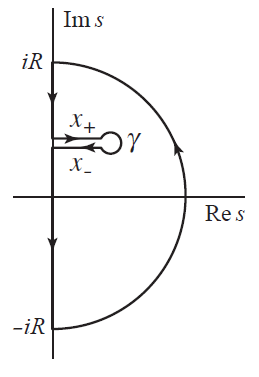
\includegraphics[scale = 0.5]{bodePlot}
  \caption{Contour integral for Bode's integral theorem with a single pole. From \cite{astrom_feedback_2010}}
\end{figure}

We can divide the integral into 3 parts:

\begin{align}
\int_{\Gamma} \log(S(s))\,ds &= \int^{iR}_{-iR}\log(S(s))\,ds + \int_{R}\log(S(s))\,ds + \sum_{k}\int_{\gamma}\log(S(s))\,ds \\
&= I_{1} + I_{2} + I_{3}
\end{align}

Now we can calculate term by term. $I_{1}$ can be written:

\begin{equation}
I_{1} = -i\int^{iR}_{iR}\log(S(i \omega))\, d\omega = -2i\int^{iR}_{0}\log(|S(i\omega|)|)\, d\omega
\end{equation}

By writing $I_{2}$ in terms of $L(s)$ and using the approximation $\log(1 + x) \approx x$ for small $x$:

\begin{equation}
I_{2} = \int_{R}los(S(s))\, ds = -\int_{R}\log(1 + L(s))\, ds \approx -\int_{R}L(s)\, ds
\end{equation}

This tends to zero faster than $1/s$, so $I_{2} \to 0$ as $R \to \infty$. Finally, we consider $I_{3}$ in terms of the three parts of the `cut-out': $X_{+}$, $X_{-}$ and $\gamma$:

\begin{equation}
I_{3} = \int_{X_{+}}log(S(s))\, ds + \int_{\gamma}log(S(s))\, ds + \int_{X_{-}}log(S(s))\, ds
\end{equation}

The integral around $\gamma$ goes to zero, leaving. Evaluating the $X_{+}$ and $X_{-}$ terms we get:

\begin{equation}
I_{3} = 2\pi i \sum_{k}\Re(p_{k})
\end{equation}

This gives:

\begin{equation}
-2 i \int^{R}_{0}\log|S(i \omega)|\, d\omega + i \sum_{k} 2 \pi \Re(p_{k})
\end{equation}

Writing $S(i \omega)$ in terms of $L(i \omega)$ and dividing through by $2i$ gives the result.

\section{Derive optimal control and cost-to-go of LQG control}
Following the presentation given in \cite{todorov2006optimal}: Optimal control of a Linear Quadratic Gaussian system gives a closed-form control law. With the control problem:
\begin{align}
\textit{dynamics: } &d\mathbf{x} = (A\mathbf{x} + B\mathbf{u})dt + Fd\mathbf{w} \\
\textit{cost rate: } &l(\mathbf{x}, \mathbf{u}) = \frac{1}{2}\mathbf{u}^{T}R\mathbf{u} + \frac{1}{2}\mathbf{x}^{T}Q\mathbf{x} \\
\textit{final cost: } &h(\mathbf{x}) = \frac{1}{2}\mathbf{x}^{T}Q^{f}\mathbf{x}
\end{align}
We seek a control law which satisfies the stochastic Hamilton-Jacobi-Bellman equations for optimal control law $\pi(\mathbf{x}, t)$ and optimal cost-to-go $v(\mathbf{x}, t)$:

\begin{align}
\pi(\mathbf{x}, t) = \arg &\min_{\mathbf{x} \in \mathcal{U}} \Big( l(\mathbf{x}, \mathbf{u}, t) +\mathbf{f}(\mathbf{x}, \mathbf{u})^{T}v_{\mathbf{x}}(\mathbf{x}, t) + \frac{1}{2}tr(S(\mathbf{x}, \mathbf{u})v_{\mathbf{xx}}(\mathbf{x}, t)\Big)  \\
-v_{t}(\mathbf{x}, t) = &\min_{\mathbf{x} \in \mathcal{U}} \Big( l(\mathbf{x}, \mathbf{u}, t) +\mathbf{f}(\mathbf{x}, \mathbf{u})^{T}v_{\mathbf{x}}(\mathbf{x}, t) + \frac{1}{2}tr(S(\mathbf{x}, \mathbf{u})v_{\mathbf{xx}}(\mathbf{x}, t)\Big)
\end{align}

Making the Ansatz for the optimal cost-to-go with some unknown $a(t)$ we hope to obtain later:
\begin{equation}
v(\mathbf{x}, t) = \frac{1}{2}\mathbf{x}^{T}V(t)\mathbf{x} + a(t)
\end{equation}
and inserting it into the HJB equation we recover the optimal control:
\begin{equation}
\mathbf{u} = -R^{-1}B^{T}V(t)\mathbf{x}
\end{equation}
This satisfies the $min_{\mathbf{u}}$ operator in the HJB equation, in which we can now equate the $\mathbf{x}$-dependent terms and obtain a formula for $\dot{V}(t)$ and $\dot{a}(t)$ to give the optimal cost-to-go.
\begin{equation}
-\dot{V(t)} = Q + A^{T}V(t) + V(t)A - V(t)BR^{-1}B^{T}V(t)
\end{equation}
This is called a continuous-time Ricatti equation.
\begin{equation}
-\dot{a}(t) = \frac{1}{2}trace(SV(t))
\end{equation}
Will give the optimal cost-to-go $v(\mathbf{x}, t)$ when integrated to give $a(t)$.

\section{The Simplex Algorithm}
Dantzig's Simplex algorithm is a linear programming algorithm for optimising a function of multiple variables given constraints on those variables. For example (from the webpage given in the question) maximising:

\begin{equation}
\max 5x_{1}+4x_{2}+3x_{3}
\end{equation}

Given the constraints:

\begin{align}
2x_{1} + 3x_{2} + x_{3}& \leq 5 \\
4x_{1} + x_{2} + 2x_{3}& \leq 11 \\
3x_{1} + 4x_{2} + 2x_{3}& \leq 8 \\
x_{1}, x_{2}, x_{3}& \geq 0
\end{align}

We contain the objective within a variable $z$:

\begin{equation}
z = 5x_{1} + 4x_{2} + 3x_{3}
\end{equation}

The constraints to the $x_{i}$ are encoded in linear combinations of the initial variables, which we call `slack variables':

\begin{align}
x_{4} &= 5 - 2x_{1} - 3x_{2} - x_{3}\\
x_{5} &= 11 - 4x_{1} - x_{2} - 2x_{3}\\
x_{6} &= 8 - 3x_{1} - 4x_{2} -2x_{3}
\end{align}

Together with the equation for $z$ this is called a dictionary for the linear optimisation problem. We can represent all this information in an augmented matrix called a `tableau', written:

\begin{equation}
\begin{bmatrix}
0 & A & I & b\\
-1 & c^{T} &0 &0
\end{bmatrix}
\end{equation}

where $A$ is the matrix of coefficients of constraints (the LHS of the constraint equations), $b$ is the values on the RHS of the constraint equations, $c$ the vector of coefficients of the objective variable and $I$ the identity matrix. We then choose a column to eliminate (the `pivot' column) and perform Gaussian elimination on the augmented matrix using this column. Continue pivoting until all the elements of $c^{T}$ are less than zero - this is an optimal solution as increasing any of the variables will decrease the objective variable. It is also possible to compute a matrix (`Gaussian pivot matrix') for each step such that multiplying the simplex tableau by this matrix will perform the desired pivot.

\section{Molecular Democracy: who shares the controls?}
From \cite{kacser_molecular_1979} Summation theorem:

Assume that the expression for the rate of a reaction is a function of (at most) the substrates $S_{i}$, inhibitors $I_{i}$, cofactors $Co_{i}$, rate constants $k_{i}$ and equilibrium constants $K_{i}$. Then the sum of the sensitivity coefficients $\mathbf{Z}_{i}$ is unity:

\begin{equation}
\sum^{n}_{i=1}\mathbf{Z}^{F_{j}}_{E_{i}} = 1
\end{equation}


We can show this by considering the situation at steady-state: the intermediate metabolite concentrations are constant. Increasing all enzymes by some small $\alpha$ doesn't change metabolite concentrations:

\begin{equation}
\frac{\delta E_{i}}{E_{i}} = \alpha \; \implies \; S_{i} = constant
\end{equation}


It does, however, change fluxes:

\begin{equation}
\frac{\delta F_{j}}{F_{j}} = \alpha
\end{equation}

Now taking partial derivatives:

\begin{equation}
\frac{dF_{j}}{F_{j}} = \sum^{n}_{i=1} \left( \frac{\delta F_{j}}{F_{j}} \middle/ \frac{\delta E_{i}}{E_{i}}  \right) \frac{dE_{i}}{E_{i}}
\end{equation}

Recognising the partial derivatives as the sensitivity coefficients $\mathbf{Z_{i}}$ and taking the limit:

\begin{equation}
\alpha = \alpha \sum^{n}_{i=1}\mathbf{Z}_{i} \; \implies \; \sum^{n}_{i=1}\mathbf{Z}_{i} = 1
\end{equation}

Connectivity theorem:
\newline
\newline
Define the elasticity coefficient:

\begin{equation}
\frac{\delta v_{i}}{v_{i}} \bigg/ \frac{\delta S_{i}}{S_{i}} \to \frac {\partial \ln v_{i}}{\partial \ln S_{i}} = \varepsilon^{v_{i}}_{S_{i}}
\end{equation}

The connectivity theorem states that:

\begin{equation}
\frac{\mathbf{Z}_{i}}{\mathbf{Z}_{j}} = -\frac{\varepsilon^{j}}{\varepsilon^{i}}
\end{equation}
 
We can see this by substituting $dv/v = dE/E$ into the definition of the elasticity coefficient for enzymes $i$ and $j$ which share a common linking metabolite and inserting this into the expression for the system flux:

\begin{equation}
\frac{dF}{F} = 0 = \mathbf{Z}_{i} \frac{dE_{i}}{E_{i}} + \mathbf{Z}_{j} \frac{dE_{j}}{E_{j}}
\end{equation}

This gives:

\begin{equation}
\mathbf{Z}_{i} \varepsilon^{i} + \mathbf{Z}_{j} \varepsilon^{j} = 0
\end{equation}

Dividing through gives the result.

\section{Derivation of the Michaelis-Menten expression}
This derivation follows that given on the webpage in the question. Consider an enzyme $E$ that catalyses a reaction from substrate $S$ to product $P$:

\begin{equation}
E + S \mathrel{\mathop{\rightleftarrows}^{\mathrm{k_{1}}}_{\mathrm{k_{-1}}}} ES \mathrel{\mathop{\rightarrow}^{\mathrm{k_{cat}}}} E + P
\end{equation}

Assume the reaction has first-order kinetics, so rate $v_{0}$ has:

\begin{equation}
v_{0} = \frac{d[P]}{dt} = k_{cat}[ES]
\end{equation}

If the reaction is at steady state, then the rate of formation of the intermediate $ES$ (LHS below) equals its rate of consumption (RHS below):

\begin{equation}
k_{-1}[ES] + k_{cat}[ES] = k_{1}[E][S]
\end{equation}

Now we find:

\begin{equation}
\frac{k_{-1} + k_{cat}}{k_{1}} = \frac{[E][S]}{[ES]}
\end{equation}

Grouping together the rate constants into one constant $K_{m} = (k_{-1} + k_{cat}/k_{1})$ and writing $[E] = [E]_{total} - [ES]$ we obtain:

\begin{equation}
K_{m} = \frac{([E]_{total} - [ES])[S]}{[ES]}
\end{equation}

Rearranging:

\begin{equation}
[ES] = \frac{[E]_{total}[S]}{K_{m} + [S]}
\end{equation}

The rate of reaction has a maximum velocity $v_{max}$ when all enzymes are saturated, i.e. $[ES] = [E]_{total}$. This means $v_{max} = k_{cat}[E]_{total}$. Substituting this into our initial equation:

\begin{equation}
v_{0} = \frac{v_{max}[S]}{K_{m} + [S]}
\end{equation}

This is the Michaelis-Menten equation. The Michaelis constant $K_{m}$ is the substrate concentration where the rate of reaction is half $v_{max}$. The reaction rate will asymptotically approach $v_{max}$ with increasing substrate saturation - the reaction rate is a rectangular hyperbola.

\bibliographystyle{nature}
\bibliography{ICDNS}

\end{document}
